\documentclass[preprint,10pt]{sigplanconf}
\usepackage[T1]{fontenc} %%%key to get copy and paste for the code!
\usepackage[utf8]{inputenc} %%% to support copy and paste with accents for frnehc stuff
\usepackage{times}
\usepackage[scaled=0.85]{helvet}
\usepackage{graphicx}
\usepackage{ifthen}
\usepackage{xspace}
\usepackage{alltt} 
\usepackage{latexsym}
\usepackage{url}            
\usepackage{amssymb}
\usepackage{amsfonts}
\usepackage{stmaryrd}
\usepackage{balance}
\usepackage{enumerate}
\usepackage[pdftex,colorlinks=true,pdfstartview=FitV,linkcolor=blue,citecolor=blue,urlcolor=blue]{hyperref}
\usepackage{xspace}


\input{macros}

\begin{document}

\conferenceinfo{WXYZ '05}{date, City.} 
\copyrightyear{2005} 
\copyrightdata{[to be supplied]} 
 
\title{Towards a flexible Pharo Compiler}

\authorinfo{Cl\'ement B\'era}
           {RMOD - INRIA Lille Nord Europe}
           {clement.bera@inria.fr}
\authorinfo{Marcus Denker}
           {RMOD - INRIA Lille Nord Europe}
           {marcus.denker@inria.fr}

\maketitle


\begin{abstract}
The Pharo Smalltalk-inspired language and environment started its development with a codebase that can be traced back to the original Smalltalk-80 release from 1983.
Over the last years, Pharo has been used as the basis of many research projects. Often these experiments needed changes related to the compiler infrastructure. However, often they did not use the existing compiler and instead implemented their own experimental solutions.
This shows that despite being an impressive achievement considering its age of over 35 years, the compiler infrastructure is showing its age. 

We identify three problems: (i) The architecture is not reusable, (ii) compilation can not be parametrized and (iii) the mapping between source code and bytecode is overly complex.

Solving these problems will not only help researchers to develop new languages, the enhanced power of the infrastructure allows many tools and frameworks to be built that are important even for day-to-day development, such as debuggers and code transformation tools.

In this paper we discuss the three problems, show how these are solved with a new Compiler model. We present an implementation, Opal, and show how Opal is used as the bases for many important tools for the everyday development of Pharo 3.
\end{abstract}


\section{Introduction}
\label{sec:intro}

A lot of research has been done with Pharo and Squeak in the past. Examples are Bytecode Manipulation with Bytesurgeon\cite{Denk06a}, Advanced  Reflection\cite{Denk07b, Roet08a, Denk08b},
Typesystems~\cite{Hald09a}, Transactional Memory\cite{Reng09a} or Omniscient Debuggers\cite{Hofe06a, Lien08b}. 

All these research experiments implemented by changing the compiler of Pharo/Squeak, and sometimes combined with virtual machine(VM)-level changes.
In contrast to VM-level changes, compiler based experiments have many advantages: The compiler is implemented in Smalltalk, therefore the standard tools and debugging infrastructure can be used. In addition, the models realized in Smalltalk tend to be far more abstract than the implementation at the VM-level.

One of the reason why Pharo exists is the idea to create a fast feedback loop for development. We revisit successful research results and integrate them back into the system. 
This way, future researchers can build on top of the results of prior work instead of always starting from scratch. 

Opal is the practical result coming out of the compiler infrastructure used for past research experiments. The code-base has therefore  seen already considerable use in experiments over the years.  

The compiler framework described in this paper is the result of revisiting the experimental code with the result of a compiler that is stable and
clean to be integrated in Pharo 3 with the goal of removing the old compiler in Pharo 4.

\subsection{The Smalltalk Compiler}
In a traditional Smalltalk system, Smalltalk code (text) is compiled to bytecode. This compilation happens on a per method basis when the programmer saves an edited method.

The Smalltalk bytecode is a traditional stack-based bytecode, the bytecode set of Pharo is taken from Squeak and therefore an extension of the original Smalltalk
80 bytecode with extensions to support block closures as implemented by the Cog VM~\cite{Mira11a}.


\begin{figure}[ht]
\begin{center}
	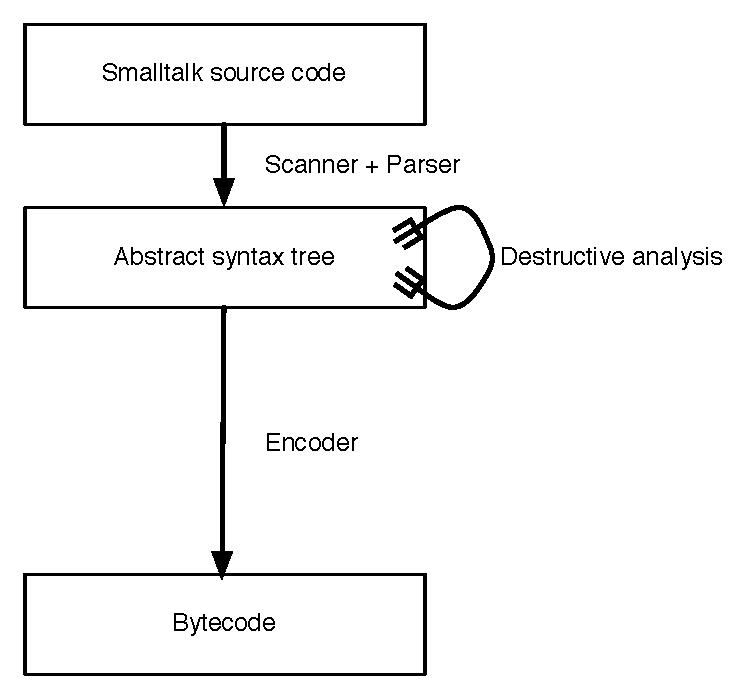
\includegraphics[width=6cm]{oldCompilerModel}
	\caption{A representation of the old compiler toolchain}
	\figlabel{oldCompilerModel}
\end{center}
\end{figure}

The Smalltalk bytecode set provides some ways for the compiler to optimize code statically: Loops and conditionals are compiled to jump instructions and conditions.

As the traditional Smalltalk system provides a decompiler from bytecode to text, no other optimizations are done. The goal is to be able to re-create  the original source
from bytecode, which would be impossible if any serious optimizations would be done.

As such, Opal right now too compiles to exactly the same bytecode as the old compiler. 

It should be noted that in a modern Smalltalk VM, there is second compiler, a so-called JIT compiler, in the VM that compiles
the bytecode to native code. This paper is not concerned at all with this VM-level compiler.

\subsection{Smalltalk Language Tools}

Besides the compiler, many IDE-level tools in Smalltalk are reasoning about code. In the following we give a short overview.

\paragraph{Refactoring Engine.}
The prime example is the Refactoring Engine \cite{Robe97a} which is the basis of all transformations
related to Refactoring. As the original AST of the Smalltalk compiler was not designed for
transformations, the RB implements its own parser and AST.

\paragraph{Syntax Highlighting.}
As any modern IDE, Pharo supports syntax highlighting in real time while the developers types. Syntax highlighting is
implemented using its own parser and representation of code, not reusing any parts of the compiler or the refactoring
engine.

\paragraph{Debugger.}
The debugger is a central tool for the Smalltalk developer. Often development happens right in the debugger. 
To support highlighting of the execution when stepping, the debugger needs to have a mapping from bytecode to source code.
This mapping can only be provided by the compiler, making the debugger reliant on the compiler in a non-trivial way.

In this paper we analyse the problems that the old compiler framework poses. We identify in Section \secref{problem} three
problems:
\begin{enumerate}
\item The architecture is not reusable,
\item The compilation can not be parametrized,
\item The mapping between source code and bytecode is overly complex.
\end{enumerate}

We present a model for a new compiler (Section \secref{contribution}) to solve these problems. After we discuss implementation details (Section \secref{implementation}, we validate the new infrastructure by
showing benchmarks and the tools that are build on top of Opal (Section \secref{validation}).


\section{Problems of the Current Compiler}
\label{sec:problem}

Pharo uses nowadays a direct child of the Smalltalk-80 original compiler. Despite being an impressive piece of work for the eighties, the architecture shows its age. As a result, the compiler framework (scanner, parser, AST) are not used by other parts of the system. For example, the refactoring engine uses its own AST.

\paragraph{Reusable architecture.} There are modularity problems in all the levels of the compilation toolchain. At the AST-level, Pharo uses different AST implementations. To be consistent (and for maintainanability purposes), there should be only one AST for the whole system, not one AST per feature. 

Then, on the semantic analysis-level, another problem is raised. The AST is dependent on the compiler to the point that the semantic analysis destroys the AST, creating artefacts only usable by the compiler. Again, the semantic analysis should be reused in the system and implemented only once. 

Lastly, at bytecode-level, no intermediate representation exists in the compiler. Therefore, the existing compiler backend can not be used elsewhere.

\paragraph{Source code mapping.} Another issue is the complexity of the debugging features.
According to the current bytecode set of Squeak and Pharo, the bytecode representation is not aware of the names of the temporary variables, but only about their indexes.
It does also not know about the highlighting range.
As the difference between the generated bytecode and the AST is huge, you have to implement a mapping between the bytecode and the AST to be able to get the temporary variable names and the highlighting range.
This mapping is complex, especially for blocks and even more so for inlined blocks.

\paragraph{Parametrized compilation.} 
Pharo developers would like to compile certain parts of the system differently, reaching from a bunch of methods up to a large panel of classes.
For example, with the old compiler a tree of classes can not be recompiled without automatic inlining of conditional messages.
Another parametrization that would be interesting is to be able to plug in different classes for the compilation passes like parsing, semantic analysis or code generation.

%Probably set the vocabulary before to cut any misinterpretation

%Constraints that influenced the solution (because the solution is not
%universal) \emph{e.g.} our requirements for a solution, possibly not all
%satisfied. They should be sound and believable. Analysis of the criteria.
%Imagine that you are another guy having this problem do the constraint
%matches yours so that you could apply the solution

%Problem
\paragraph{Problem Summary:}
How can we have a flexible compiler with reusable and high-level intermediate representations?

The Opal compiler offers a solution to these problems. The flexibility comes from its pluggable architecture: you can easily change the object managing a part of the compilation chain. Opal relies on reusable representations as the RB AST or the bytecode-level intermediate representation (IR). 

\section{Opal: A Layered Compiler Chain}
\label{sec:contribution}

In this section we present the design of Opal from a high-level point of view.

\subsection{The Opal Model}

\begin{figure}[ht]
\begin{center}
	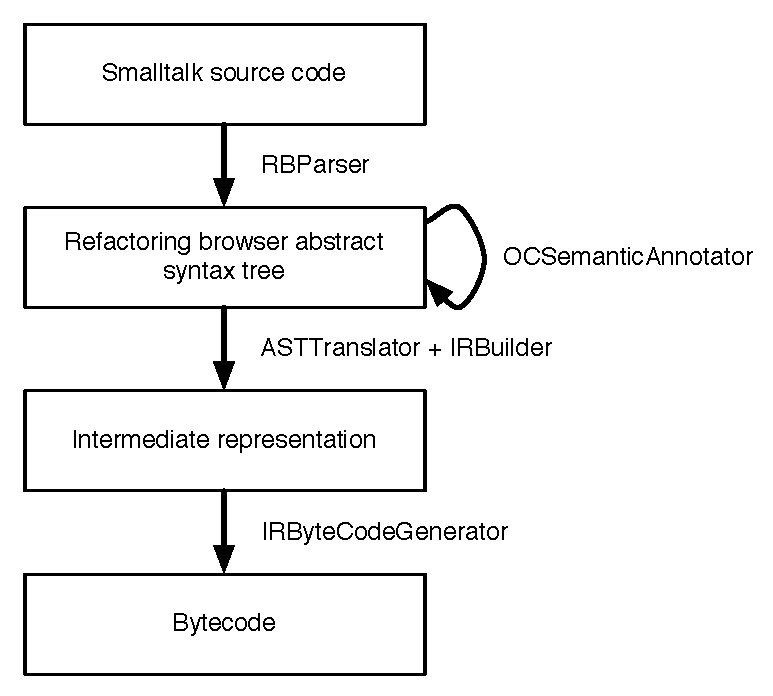
\includegraphics[width=6cm]{OpalModel}
	\caption{The Opal compilation toolchain's four stages}
	\figlabel{OpalModel}
\end{center}
\end{figure}


\paragraph{Explicit compilation passes.}
As shown in Figure \ref{fig:OpalModel}, the smalltalk code is parsed with RBParser to the RB AST. Then the OCSemanticAnalyser annotates it.
The ASTTranslator visits it, building the IR with IRBuilder. Lastly, the IRByteCodeGenerator generates bytecode out of the IR.

\subsection{Annotated RB AST: a Reusable Code Representation}

Instead of creating a whole new representation, Opal reuses the AST from the refactoring browser. In addition, the semantic analysis does not change the AST, but only annotates it. This guarantees the reusability of the representation. 

On the figure \figref{RBModel}, we can see the class diagram of the RB AST. All nodes inherit from the same superclass \ct{RBProgramNode}. This way, they all have two main states: properties, which is a dictionary for annotations and parent, which is a back pointer to the outer node.

\begin{figure}[ht]
\begin{center}
	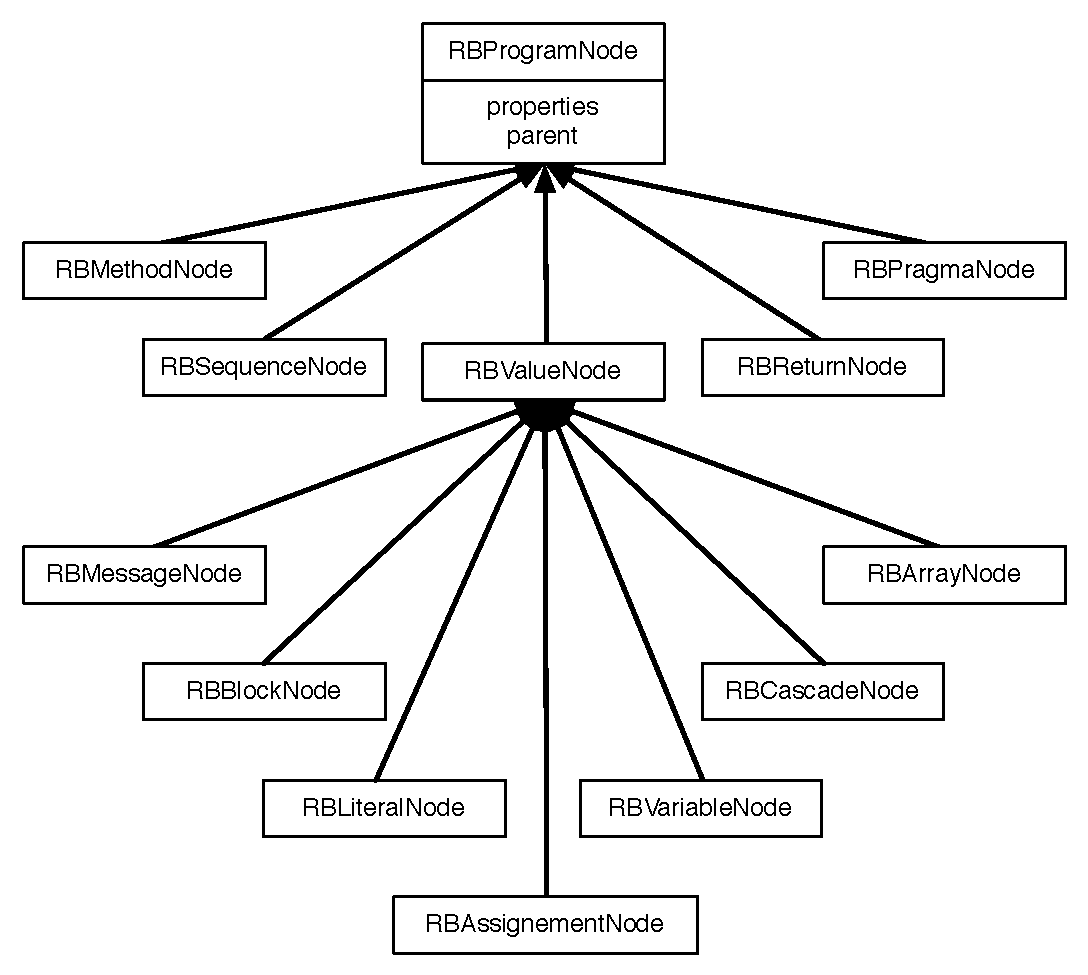
\includegraphics[width=8cm]{RBModel}
	\caption{The refactoring browser AST class diagram}
	\figlabel{RBModel}
\end{center}
\end{figure}


\subsection{Compilation Context}

\begin{figure}[ht]
\begin{center}
	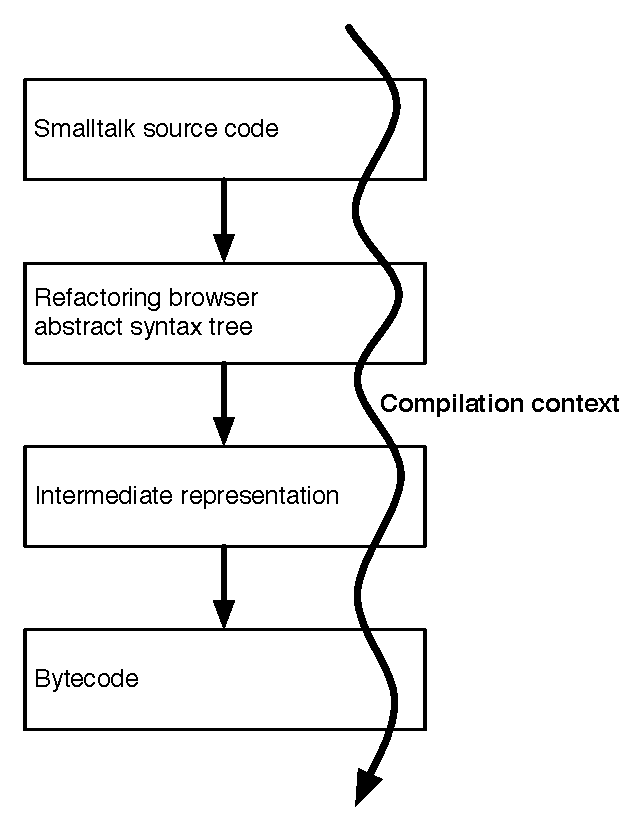
\includegraphics[width=6cm]{OpalCompilationContext}
	\caption{The compilation context in Opal compilation toolchain}
	\figlabel{OpalCompilationContext}
\end{center}
\end{figure}

When you compile a method to bytecode, you want to pass some objects along the compilation chain. For example, the old compiler used to pass:

\begin{itemize}
	\item the requestor: this object corresponds to the UI element that holds the text to compile. 
This very useful because it permits for example to write error messages directly in the morph text instead of raising an error.
For example, if you compile \ct{[:y | [:y | y ] ] }, you will get  \ct{[:y | [ Name already defined ->:y | y ] ] } instead of an error.
	\item the failBlock: is executed when the compilation fails in interactive mode. Usually this happens because the source code was incorrect and an error was raised. 
\end{itemize}

All this information is needed. But the issue with this approach is that it requires to always pass along these object through the whole compilation toolchain.
 The resulting methods with excessive numbers of arguments are hard to maintain and not nice to use. For example, we have in the old compiler:
\begin{code}{}
Parser>>#parse:class:noPattern:context:notifying:ifFail:
Compiler>>#compileNoPattern:in:context:notifying:ifFail:
\end{code}

To increase the modularity of Opal, we needed to add even more arguments, most of them being booleans. We decided to add the \ct{CompilationContext} object. This object holds all these arguments and in general all information that is of interest in later
phases of the compiler. As Figure \ref{fig:OpalCompilationContext} shows, the context is passed through to the whole compilation chain.

\subsection{IR: An Explicit Intermediate Representation}
We discuss the intermediate representation  (IR) of the Opal Compiler. The following shows the class hierarchy of the IR:

\begin{code}{}
IRInstruction
        IRAccess
                IRInstVarAccess
                IRLiteralVariableAccess
                IRReceiverAccess
                IRTempAccess
                        IRRemoteTempAccess
                IRThisContextAccess
        IRJump
                IRJumpIf
                IRPushClosureCopy
        IRPop
        IRPushArray
        IRPushDup
        IRPushLiteral
        IRReturn
                IRBlockReturnTop
        IRSend
        IRTempVector
IRMethod
IRSequence
\end{code}

This intermediate representation is modeling the bytecode yet abstracts away from details. It forms a Control Flow Graph (CFG). IRInstructions are forming basic blocks using IRSequence, these sequences are concatenated by the last instruction which is an IRJump.


Opal has an explicit low-level representation for three main reasons.
Firstly, it gives to the user the possibility to easily transform the bytecode. 
Secondly, it simplifies a lot the debugging capabilities implementation of the system, as explained in section \secref{opalDebugging}.
Lastly, this representation provides an abstraction over the bytecode, letting the whole compilation chain of Opal independent of details of the bytecode representation. A dedicated backend visits the IR (IRBytecodeGenerator, as shown in Figure~\ref{fig:OpalModel}).

\subsection{Debugging Features}

The AST with semantic analysis and its IR, provide the basis to map between all the representations. For example, mapping between bytecode offset and text. Details are explained in Section~\ref{sec:tempNamesMapping}.


\section{Opal Implementation Details}
\label{sec:implementation}

In this Section, we will present some of the implementation details of Opal. We will discuss two aspects: first the compilation context and how it enables Opal to be parametrizable and pluggable. Second we discuss in detail the infrastructure put in place for mapping text with AST, IR and low-level offsets in compiled code.

\subsection{Compilation Context}

In this subsection, we describe the compilation context and its capabilities. The compilation context is an object that holds state that is of interest to later passes done by the compiler. The class definition is shown here:

\begin{code}{}
Object subclass: #CompilationContext
    instanceVariableNames: 'requestor failBlock noPattern class 
                            category logged interactive options 
                            environment parserClass semanticAnalyzerClass 
                            astTranslatorClass bytecodeGeneratorClass'
    classVariableNames: ''
    poolDictionaries: ''
    category: 'OpalCompiler-Core-FrontEnd'
\end{code}

The instance variables all help to make Opal more customizable and to change the compilation chain. We present them one by one.

\paragraph{Basic data.}

\begin{description}
\item[requestor]: this object corresponds to the user interface element that holds the text to compile.
\item[failBlock]: this block is executed when the compilation fails.
\item[noPattern]: this boolean tells if the text to compile starts with the method body or by the method selector.
\item[class]: the class of the compiled object to know how to compile accesses to instance variables.
\item[category]: the category where the compiled method should be put.
\item[logged]: will the new compiledMethod creation be logged in the changes file.
\item[interactive]: does this compilation happen in interactive mode (Warnings are raised and stops the compilation) or in non interactive mode (Warnings are shown on console logging and does not stop the compilation).
\item[environment]: points to the Smalltalk environment (usually an instance of Smalltalk image) where you compile. This is used for example for remote compilation.
\end{description}

\paragraph{Compiler options.}

The Opal compiler proposes options.
A programmer can specify them either on a per class basis by overriding the \ct{compiler} method or on method basis with a pragma. 
These options are passed with the compilation context through all stages of the compiler and can be read and reacted upon on any level.
The first set of options concern optimizations of control-structures and loops:


\begin{itemize}

\item  \begin{code}{}
optInlineIf
optInlineIfNil
optInlineAndOr
optInlineWhile
optInlineToDo
optInlineCase
\end{code}

This set of options controls automatic inlining of some message, such as \ct{ifTrue:} and \ct{and:}.

\item \ct{optLongIvarAccessBytecodes }

This option forces the compiler to generate long bytecodes for accessing instance variables.
It is used for all classes related to MethodContext to support c-stack to Smalltalk stack mapping.

\item \ct{optOptimizeIR}

This option controls the activation of some basic IR optimisations.

\end{itemize}

\paragraph{Compiler Plugins.}

In some cases it can be useful to replace parts of the compilation chain. 
Therefore the programmer can change which class is used for each compilation phase.
One can redefine:

\begin{description}
\item[parserClass:] change the class that parses Smalltalk code and returns an RB AST. For instance a scannerless Parser could be used instead.
\item[semanticAnalyzerClass:] change the class that is performing the semantic analysis on the RB AST nodes.
\item[astTranslatorClass:] change who translates the RB AST to Opal IR intermediate representation.
\item[bytecodeGeneratorClass:] change the generator class used to create bytecode from the Intermediate representation. This is especially useful when experimenting with new bytecode sets.
\end{description}

\subsection{Opal Debugging Features}
\label{sec:opalDebugging}

A central feature of any Smalltalk is its advanced debugger. To be able to implement a stepping debugger, there needs to be a mapping between the program counter on the bytecode-level and the text that the programmer wrote.
In addition, we need to be able to access temporary variables by name.

\subsubsection{Debugger Highlighting}

The AST nodes know their source intervals as they are recorded when parsing. Then, each IR instruction knows the AST node that generated them. Lastly, from each bytecode you can get the IR quite easily, as each IR node knows the index of the corresponding generated bytecode.

\begin{figure}[ht]
\begin{center}
	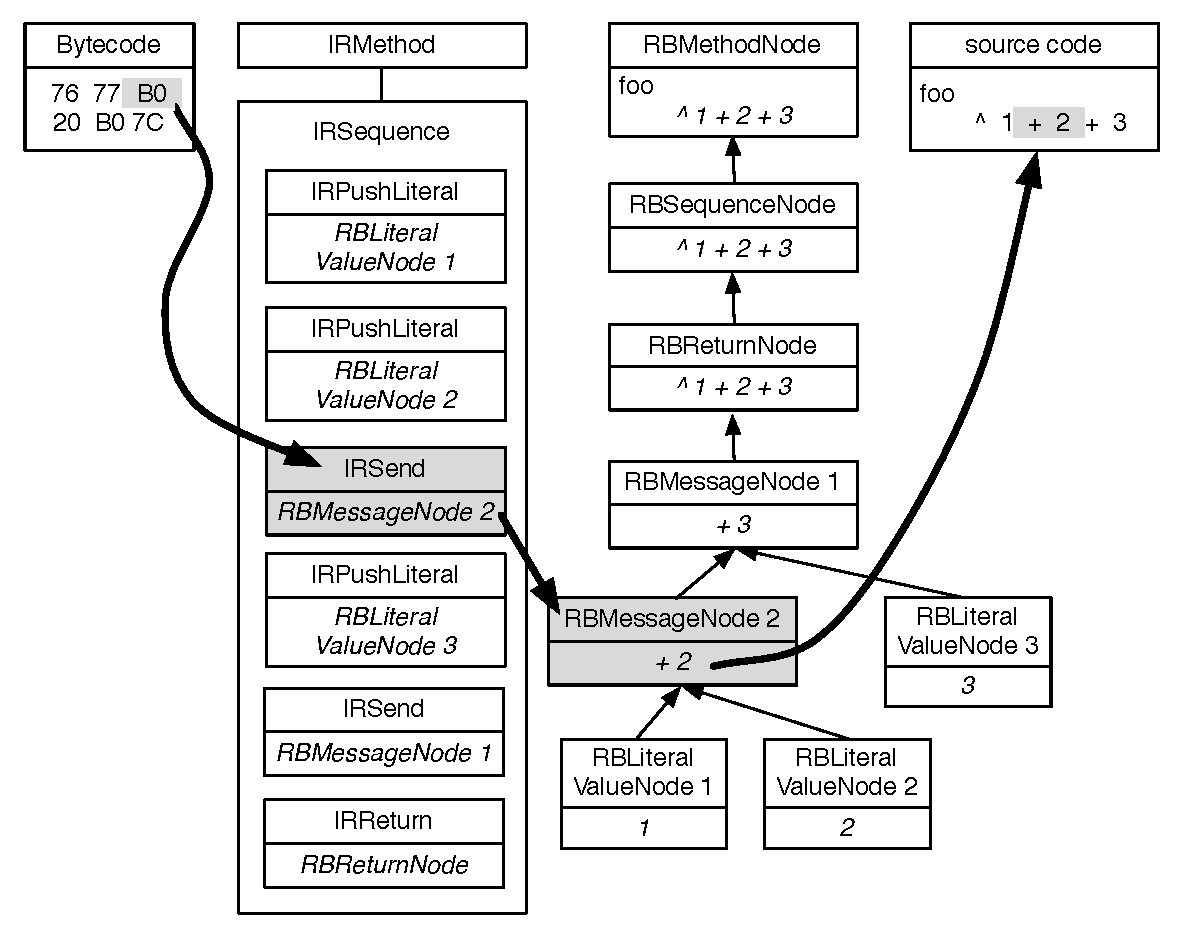
\includegraphics[width=9cm]{BCToSource}
	\caption{Bytecode to source code highlighting}
	\figlabel{BCToSource}
\end{center}
\end{figure}

Therefore the mapping can be done easily at AST/IR-level. Figure~\ref{fig:BCToSource} shows a complete example of mapping an offset in the bytecode to the source.
The idea is to generate the AST and IR from the compiled method, then to map from bytecode to IR to AST and lastly to the source interval. 
So the mapping does not build up special data structures, but instead relies on annotations on the AST and the IR that are generated by the compiler.
It should be noted that we need to do a full compilation of the method from the sources to get the correct AST and IR mapping.

\subsubsection{Temporary Name Mapping}
\label{sec:tempNamesMapping}

Temporary variables are accessed through an offset. This is done for performance. For a simple temporary variable, the runtime representation of the method (called context) uses this offset to access the value of the variable. Moreover, Pharo supports blocks (commonly called closures). As these closures can live longer than their enclosing context, they also need their own runtime representation (context). Variables shared between closures and their enclosing contexts are stored in a heap allocated array named tempVector. Here is an example of a method with a block and shared variables:

\begin{code}{}
SomeRandomClass>>foo
        | temp1 temp2 |
        temp1 := #bar.
        [ | closureTemp |
        closureTemp := #baz.
        temp2 := closureTemp ] value.
        \ret temp2
\end{code}

We see in Figure \ref{fig:temps} that the offset of the temporary variable \ct{temp1} is 2 in the method context. \ct{temp2}, being shared by both the block and the method context, is stored in a temp vector. So its offset, while being accessed from the block or the method context, is 1 to reach the temp vector, then 1 which correspond to the offset in the temp vector.

\begin{figure}[ht]
\begin{center}
	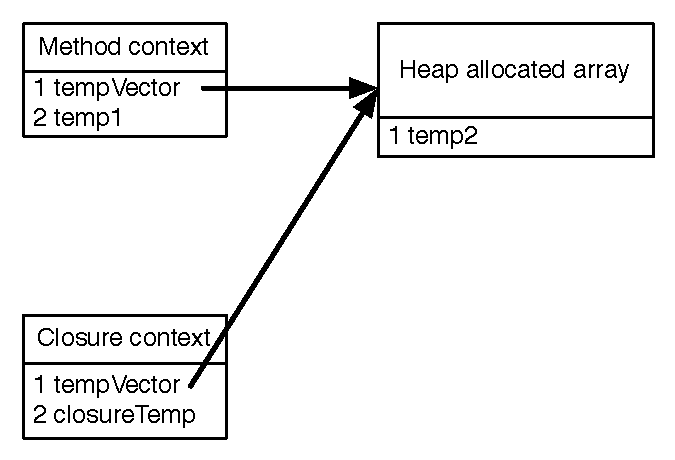
\includegraphics[width=6cm]{temps}
	\caption{Runtime temporary variable storage}
	\figlabel{temps}
\end{center}
\end{figure}

To speed up the execution, one optimization is implemented. The temporary variables that are read-only in the closure are not stored on the external array but passed to the block context similarly to an argument. 

Temporary name mapping is the correspondence between these offsets and the variable name. This mapping can be complex: in Smalltalk, one can have several nested blocks in a method and in each block there might be some read-only or written temporaries. This mapping is used for debugging (debugger and inspectors).

As an example for inspecting a context, the following code presents a simple temp access:

\begin{code}{}
SomeRandomClass>>example
        | temp |
        temp := #bar.
        \ret temp
\end{code}

The offset of the temporary variable \ct{temp} is 1. Therefore, when we inspect a context, the result is just an inspector on an object that has offsets, as we see in \figref{inspectorIndex}.

\begin{figure}[ht]
\begin{center}
	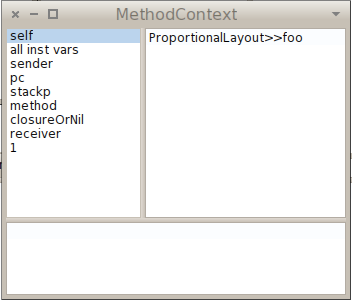
\includegraphics[width=5cm]{inspectorIndex}
	\caption{A basic inspector on a context}
	\figlabel{inspectorIndex}
\end{center}
\end{figure}

Programmers do not want to debug contexts with indexes of temporaries, but with temporary names (\figref{inspectorName}). 
\begin{figure}[ht]
\begin{center}
	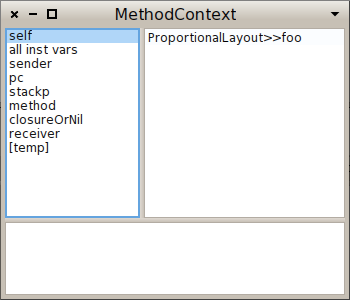
\includegraphics[width=5cm]{inspectorName}
	\caption{A specific inspector on a context}
	\figlabel{inspectorName}
\end{center}
\end{figure}

\paragraph{Temporary Names with Opal.}

Similarly to the highlighting implementation, we want to reify all needed information at the AST-level. We leverage the information added to the AST in the semantic analysis phase of the compiler.
This includes objects modeling temporary names and offsets as well as so called scopes for each method or block AST node. These scopes store defined variables and are used for mapping names to the objects describing the variables. Each node can therefore access the corresponding scope due to the parent relationship in the AST. 

In figure \ref{fig:inspectorName}, we can click on the \ct{[temp]} entry. This displays on the right panel the value. To do this, the context needs to know to which offset correspond the temporary name \ct{temp}. The context knows in this case for the temporary variable offset the associated value. It knows that offset 1 is associated to the value \ct{\#bar}. The context, being a representation of the method, can access its corresponding method AST node. The node then provides through scopes the offset information about the variable. Of course, this simple example becomes exponentially complex when we have multiple closures inside the methods with shared variables that need to be stored in temp vectors.

The temporary name mapping, now working on AST-level, works the same way for optimized blocks (\ct{to:do:}, \ct{ifTrue:ifFalse:}, \ct{ifNil:ifNotNil:}, \ct{and:}, \ct{or:}) and non optimized blocks.

\section{Validation}
\label{sec:validation}

We have discussed three problems of the old compiler infrastructure in Section~\secref{problem}. We will show in the following how the new design of Opal solves
the problems.

To show that the resulting implementation is usable in practice, we show benchmarks of compilations speed.


\subsection{Problem 1: Reusable Architecture}
\label{sec:reusableArchitecture}

Pharo 3 is moving many subsystems to use parts of the Opal Infrastructure. We highlight some of them.

\paragraph{AST-interpreter.} We implemented a complete AST-interpreter on top of the annotated AST. The AST-interpreter is written in Pharo, permitting to prove the reusability of the annotated AST. The interpreter is able to interpret all the tests of the Pharo Kernel, and they all pass.

\paragraph{Hazelnut.} In the case of Hazelnut~\cite{Casa11a}, a bootstrap of a new Pharo image from sources, Guillermo Polito uses Opal for the flexible features of the semantic analysis tool. As he needs to compile some smalltalk code not for the current Pharo environment, but for a remote image, he needs to change the way variables are resolved. He implemented his own semantic analyzer, with different bindings for variables, replacing the one from Opal. Lastly, he used Opal to compile the methods, with a different semantic analyzer that the default Opal one.

\paragraph{Metalinks.} Reflectivity is a tool to annotate AST nodes with Metalinks. A Metalink annotates an AST node. Metalinks can be executed before a node, instead a node, after a node, if the execution of a node yields an error or if the execution of a node yields no error. Once the AST of a method is annotated with some metalinks, a method wrapper replace the method to handles the compilation of an expanded version of the AST that takes metalink into account and then install the resulting method. This tool rewrites the AST nodes according to their metalinks. The new AST is recompiled thanks to Opal.

\paragraph{Class builder.} In the new Pharo class builder~\cite{Verw11a, Verw11b}, optimizations are done to avoid class hierarchy recompilation.  On the low-level, this means that you have to shift the instance variable offset to fit to the new slot class model. This is done, in the case of a compilation with Opal, with IR transformations.

\paragraph{Smart suggestions.} While we are coding we usually want to apply actions on the current edited element. For example if we have selected a variable we may want to rename it. To do this, IDEs often have large menus, including the correct feature,usually with lot of options that do not apply to the selected element. 

Smart suggestions shows only the options that you can apply to the selected AST node. We use the current AST to do this through \ct{RBParser>>\#parseFaultyMethod:} and the Opal compiler Semantic Analysis. The best AST node corresponding to the selected text is calculated. Then the available suggestions are provided. The Opal semantic analysis provides the nature of a variable: temporary, instance or class to refine the suggestions.

\paragraph {Node navigation.} Sometimes while browsing code we think in programming terms instead of text. For example we think in a message send or a statement instead of word, spaces or symbols. The idea is to use context information and let the programmer navigate the code thinking in those terms. In order to do this we find the best AST node and offer navigations in different directions:

\begin{description}		
\item[Parent:] The node that contains the selected one. For example if we have the code \ct{'aNumber between: anotherNumber'} and we are selecting the variable anotherNumber if we navigate to the parent the IDE highlights the message.
\item[Sibling:] The node in the same level that the selected. For example in a temporary variables definition: \ct{'| one two three |'} if we are in the variable one we can go to the siblings two or three.
\item[Child:] Node contained by the selected. For example if we in a message send: \ct{'aNumber between: anotherNumber'} we will go the parameter anotherNumber.
\end{description}

\paragraph{Syntax highlighting as you type.} We want to color the code we are writing using all the available information, in order to be able to select the scope where we are or to show associated information for a specific piece of code. To do that we use the AST and the semantic analysis (we need the semantic analysis because we want to show different kinds of variables with different colors, like undeclared variables), through the \ct{RBParser>>\#parseFaultyMethod:} and \ct{RBParser>>\#parseFaultyExpression:} to obtain the AST representation. The implementation is simple because we can define a new visitor defining the coloring algorithm. Once we define the coloring from each syntax representation we just visit the tree.

\subsection{Problem 2: Source Mapping}
To validate the new implementation of source code mapping, we use it as the basis for the debugger. Instead of implementing a dedicated map for the debugger (DebuggerMethodMap), we forward all requests to the AST (which is cached by the system). To test the performance, we perform a simple benchmark.
We print the error message that prints the whole stack. This prints for each stack frame all the variables:

\begin{code}{}
String streamContents: [ :str | thisContext errorReportOn: str ]
\end{code}

We execute this code in Pharo 1.4 which had a limited caching for the debugger map, as well as in Pharo 3 for both the old and the new compiler:
\vspace{0.2cm}

\begin{center}
\begin{tabular}{|l|l|}
  \hline
Pharo 1.4: &11.7 per second \\
\hline
Pharo 3 old: & 6.13 per second \\
\hline
Pharo 3 new: & 51.7 per second \\
  \hline
\end{tabular}
\end{center}

As we can see, the Opal strategy of using the annotated AST structure faster than the old strategy.

\subsection{Problem 3: Parametrized Compilation}

\paragraph{No automatic inlining.}
To prove the flexibility of the Opal compiler, a good example is not to inline some messages in some classes or methods of the system. As an example, we can advice the compiler to not inline the if statement with a pragma. With the old compiler, the if condition, sent on a non boolean object, as a symbol, raises a \ct{NonBooleanReceiver} error. On the opposite, with Opal compiler, the if condition, also sent on a symbol, raises a \ct{MessageNotUnderstood} error.

\begin{code}{}
MyClass>>foo
        <compilerOptions: - optInlineIf>
        ^ #myNonBooleanObject ifTrue: [ 1 ] ifFalse: [ 0 ]
        
MyClass new foo 
"With the old compiler, raises a runtime error NonBooleanReceiver"
"With Opal compiler, raises a MessageNotUnderstood error"
\end{code}

This is useful for different reasons. For example, researchers might want to experiment with new boolean implementations. They could want a boolean system with true, false and maybe. In this case, they needed to implement the new boolean messages with different names, creating a non readable smalltalk code, because they were not able to use the selector \ct{ifTrue:}, \ct{ifFalse:} or other optimized constructs. Other examples are proxies for booleans, symbolically executing code for type information and others.

The downside is that the non-optimized code is just produced for the methods or classes explicitly compiled with this option. To scale this to all code of the system, we recompile non-optimized code when a \ct{mustBeBoolean:} exception is raised. The nice property of this solution is that it only slows down the case where an optimized construct is called on a non-Boolean object. 

\subsection{Compilation Benchmarks}\label{sec:bench}

Even though the Opal model is introducing an Intermedia Representation (IR) and using multiple visitor passes, the resulting compiler is comparable in speed.

The benchmarks were run on a MacBook pro, on Mac OS X (Version 10.8). The machine had 8 Gb of RAM (1600MHz DDR3) and a Intel Core i5 processor of 2.5 Ghz. The SMark framework provides a precise average time of each benchmark run including error margin.

\paragraph{Compilation Speed.}

We first compare the two compilers with regard to compilation speed when recompiling classes. This exercises the whole compiler toolchain from parser down to bytecode generation and therefore gives a real world view on compilation speed. In the following table we compare recompiling the whole image and recompiling Object class:
\vspace{0.2cm}
\begin{center}
\begin{tabular}{|l|c|r|}
  \hline
  Recompile & Opal Compiler & Old Compiler  \\
  \hline
  Object class  (ms) & 296.66 $\pm$ 0.98 & 222.9 $\pm$ 2.4 \\
  Whole image  (ms)  & 72120 $\pm$ 189   & 49908 $\pm$ 240 \\
  \hline
\end{tabular}
\end{center}

As we can see, the factor between the compilers is around 1.4. Considering that Opal generates a reusable AST with annotations for semantic analysis and uses
a dedicated IR representation for the bytecode generation, this performance is acceptable. Especially considering that we can use the low-level IR backend
in cases where speed matters, as the next benchmark shows.

\paragraph{IR Benchmarks.}

The intermediate representation of Opal allows the programmer to manipulate the high-level IR instead of the low-level bytecode, AST or text. Manipulating bytecode
directly is not practical due to hard coded jump offsets and the need to create new method objects if things like number of literals or the max depth of the stack changes.
Using the high-level text or AST model for manipulating code can lead to performance problems, even when using the faster old compiler. An example for this is recompilations of class hierarchies when adding instance variables high up in the class hierarchy.

Opal provides the possibility to manipulate the IR representation instead. To assess the performance, we benchmark the speed of the IR backend. We show the times for

\begin{itemize}
\item decompiling bytecode to IR,
\item a full IR based roundtrip of decompiling and regenerating bytecode,
\item generating bytecode from IR (difference of the first two).
\end{itemize}

All these are done on all methods of the complete system.

\vspace{0.2cm}
\begin{center}
\begin{tabular}{|l|c|r|}
  \hline
BC -> IR (ms) & BC -> IR -> BC (ms) & IR -> BC (ms) \\
  \hline
  2827.2 $\pm$ 4.0 & 10533 $\pm$ 13 & 7706 $\pm$ 17\\ 
  \hline
\end{tabular}
\end{center}

The benchmarks prove that manipulating IR is much faster than recompiling source code, both with the old or the new compiler. We can
regenerate the whole bytecode of the Pharo 3 image in just 10 seconds instead of 50 seconds when recompiling with the old compiler.

This fast way to manipulate methods will be used by the new class builder when adding instance variables.

\paragraph{Runtime Speed.}
It should be noted that as the compiler generates the same bytecode, execution speed of the generated code is identical. We do therefore not provide any benchmarks.


\section{Related Work}
\label{sec:related}
Smalltalk like languages implement a compiler from text to bytecode in Smalltalk and make it available reflectively. This is not the case
with many other languages. In most languages, the compiler is a stand-alone application not visible for compiled programs. As such, all the compiler, IDE
and tools are seen as distinct and sharing implementations between them is not common. In turn, compiler frameworks that enable experiments are done
as external tools without the goal of replacing the main compiler of the language.

Polyglot~\cite{Nyst03a} is an extensible compiler framework that supports the easy creation of compilers for languages similar to Java.
A newer example is JastAdd~\cite{Ekma07b}, a compiler framework for Java that is build using a special Java-like AOP language.
It has seen a lot of use in recent implementations of AOP systems in Java.

All Smaltalk-like languages contain a compiler very similar to the old Compiler of Pharo. It is available in the language, but changing it is difficult. The easiest way to reuse the compiler is to copy the code and change it. And example of this is the Tweak extension of Smalltak used in Croquet~\cite{Smit03}.

\section{Future Work and Conclusion}
\label{sec:conclusion}

In this paper we have presented Opal, a new Compiler infrastructure for Pharo. Opal solves some problems that where found when using Pharo for 
numerous research prototypes: (i) The architecture is not reusable, (ii) compilation can not be parametrized and (iii) the mapping between source code and bytecode is overly complex. As shown, Opal solves these problem by being bases on a modular design using a compilation context and keeping the mapping explicit.

We have validated Opal by presenting benchmarks and shown a number of tools and frameworks that are build using it. Opal is already used as the default compiler  of Pharo 3.

There are many possible direction for future work, for example:

\begin{description}
\item[Compilation time optimizations.] As seen in Section \secref{bench}, Opal compiler is now 1.4 times slower than the old one. With this, Opal is already fast enough for productive use. However, we plan to conduct extensive profiling and optimization passes after the compiler has been integrated in Pharo 3.

\item[Optimizations on IR.] Currently, optimizations are done by the \ct{ASTTranslator}. For example, the inlining of block for \ct{ifTrue:} or \ct{whileTrue:} is done by analyzing the AST. However, the AST makes it hard to analyze since there is no explicit representation of control flow. Therefore, the correct place for these optimizations would be on the IR-level as the IR is a CFG (Control Flow Graph). We plan to simplify the AST to IR translation and to move the optimizations to the IR-level.

\item[Experiment with Opal.] The flexible features of Opal permits to conduct experiment more easily. We would like to experiment statically available information for optimizations. For example, it is easy to inline message sends to globals. In addition, simple limited type inference schemes are interested to explore.
\end{description}

\subsection*{Acknowledgements} We thank Gisela Decuzzi for her work and comments about AST based tools, Jorge Ressia for his work on porting Opal to the new closure model and Anthony Hanan for creating the ClosureCompiler project years ago that was the starting point for the explorations that became Opal. We thank St\'ephane Ducasse and Camillo Bruni for their reviews.

This work was supported by Ministry of Higher Education and Research, Nord-Pas de Calais Regional Council, FEDER through the 'Contrat de
Projets Etat Region (CPER) 2007-2013',  the Cutter ANR project, ANR-10-BLAN-0219 and the MEALS Marie Curie Actions program FP7-PEOPLE-2011-
IRSES MEALS. 

% \bibliographystyle{plain}
% \bibliography{foo.bib}
\balance
\bibliographystyle{alpha}
\bibliography{others,rmod}
\end{document}

%%% Local Variables: 
%%% coding: utf-8
%%% mode: latex
%%% TeX-master: "main"
%%% TeX-PDF-mode: t
%%% End:
